
                                                                               \documentclass[tikz]{standalone}
\usepackage{lmodern}
\usepackage[algoruled,vlined,linesnumbered,titlenotnumbered,noend]{algorithm2e}
\usepackage{color,amsmath,bm,bbm,stmaryrd,amssymb,pifont,bbding}
\usetikzlibrary{backgrounds}
\usetikzlibrary{calc} 

\usetikzlibrary{shapes}
\usetikzlibrary{shadows}
\usetikzlibrary{decorations.pathmorphing}
\usetikzlibrary{decorations.text}
\usetikzlibrary{decorations}
\usetikzlibrary{arrows,bending}
\usetikzlibrary{shapes.arrows}
\tikzset{nobg/.style={show background rectangle,background rectangle/.style={opacity=0}}}


\input ../../styles
\input ../../globalcomm
\input ../../localcomm
\usetikzlibrary{arrows, shapes.gates.logic.US, calc}

  \tikzstyle{bddnode}=[draw,rectangle,rounded corners=2mm]
  \tikzstyle{aops}=[pos=0.9,below,yshift=0mm,xshift=-2mm]
\begin{document}



\begin{tikzpicture}
\node[] at (0,0)
     {
       $=$
       };
\end{tikzpicture}

\begin{tikzpicture}
\node[] at (0,0)
     {
       $0$
       };
\end{tikzpicture}

\begin{tikzpicture}
\node[] at (0,0)
     {
       $1$
       };
\end{tikzpicture}


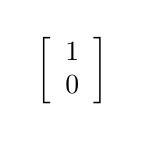
\begin{tikzpicture}
\node[] at (0,0)
     {
       $\left[
         \begin{array}{c} 1\\0\end{array}
             \right]$
       };
\end{tikzpicture}


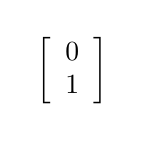
\begin{tikzpicture}
\node[] at (0,0)
     {
       $\left[
         \begin{array}{c} 0\\1\end{array}
             \right]$
       };
\end{tikzpicture}


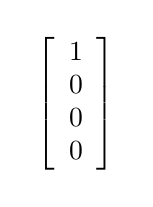
\begin{tikzpicture}
\node[] at (0,0)
     {
       $\left[
         \begin{array}{c} 1\\0\\0\\0\end{array}
             \right]$
       };
\end{tikzpicture}


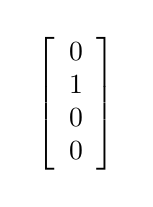
\begin{tikzpicture}
\node[] at (0,0)
     {
       $\left[
         \begin{array}{c} 0\\1\\0\\0\end{array}
             \right]$
       };
\end{tikzpicture}

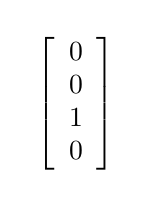
\begin{tikzpicture}
\node[] at (0,0)
     {
       $\left[
         \begin{array}{c} 0\\0\\1\\0\end{array}
             \right]$
       };
\end{tikzpicture}

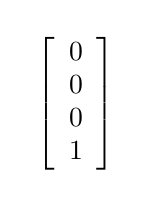
\begin{tikzpicture}
\node[] at (0,0)
     {
       $\left[
         \begin{array}{c} 0\\0\\0\\1\end{array}
             \right]$
       };
\end{tikzpicture}


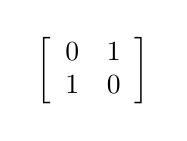
\begin{tikzpicture}
\node[] at (0,0)
     {
       $\left[
         \begin{array}{cc} 0&1\\1&0\end{array}
             \right]$
       };
\end{tikzpicture}

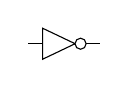
\begin{tikzpicture}
  \node[not gate US, draw,name=gate] {};
  \draw($(gate.west)+(-5pt,0pt)$) -- (gate.west);
\draw($(gate.east)+(4pt,0pt)$) -- ($(gate.east)+(9pt,0pt)$);
\end{tikzpicture}

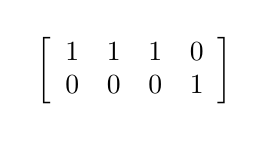
\begin{tikzpicture}
\node[] at (0,0)
     {
       $\left[
         \begin{array}{cccc} 1&1&1&0\\0&0&0&1\end{array}
             \right]$
       };
\end{tikzpicture}



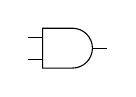
\begin{tikzpicture}
  \node[and gate US, draw,name=gate] {};
  \draw($(gate.west)+(-5pt,4pt)$) --($(gate.west)+(0pt,4pt)$);
  \draw($(gate.west)+(-5pt,-4pt)$) --($(gate.west)+(0pt,-4pt)$);
  \draw($(gate.east)+(0pt,0pt)$) -- ($(gate.east)+(5pt,0pt)$);
\end{tikzpicture}

\begin{tikzpicture}
\draw (0pt,0pt) -- (40pt,0pt);
\draw (0pt,-20pt) -- (40pt,-20pt);
\draw (20pt,0pt) -- (20pt,-22.5pt);
\node[circle,fill,inner sep=0pt,minimum size=2pt] at (20pt,0pt){};
\node[circle,draw,inner sep=0pt,minimum size=5pt] at (20pt,-20pt){};

\end{tikzpicture}


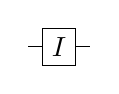
\begin{tikzpicture}
  \node[draw,name=gate] {$I$};
  \draw($(gate.west)+(-5pt,0pt)$) -- (gate.west);
\draw($(gate.east)+(0pt,0pt)$) -- ($(gate.east)+(5pt,0pt)$);
\end{tikzpicture}

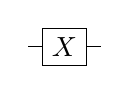
\begin{tikzpicture}
  \node[draw,name=gate] {$X$};
  \draw($(gate.west)+(-5pt,0pt)$) -- (gate.west);
\draw($(gate.east)+(0pt,0pt)$) -- ($(gate.east)+(5pt,0pt)$);
\end{tikzpicture}

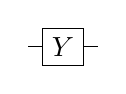
\begin{tikzpicture}
  \node[draw,name=gate] {$Y$};
  \draw($(gate.west)+(-5pt,0pt)$) -- (gate.west);
\draw($(gate.east)+(0pt,0pt)$) -- ($(gate.east)+(5pt,0pt)$);
\end{tikzpicture}

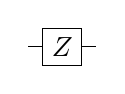
\begin{tikzpicture}
  \node[draw,name=gate] {$Z$};
  \draw($(gate.west)+(-5pt,0pt)$) -- (gate.west);
\draw($(gate.east)+(0pt,0pt)$) -- ($(gate.east)+(5pt,0pt)$);
\end{tikzpicture}

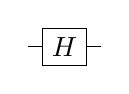
\begin{tikzpicture}
  \node[draw,name=gate] {$H$};
  \draw($(gate.west)+(-5pt,0pt)$) -- (gate.west);
\draw($(gate.east)+(0pt,0pt)$) -- ($(gate.east)+(5pt,0pt)$);
\end{tikzpicture}


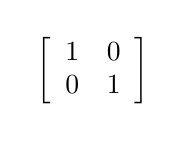
\begin{tikzpicture}
\node[] at (0,0)
     {
       $\left[
         \begin{array}{cc} 1&0\\0&1\end{array}
             \right]$
       };
\end{tikzpicture}


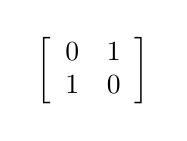
\begin{tikzpicture}
\node[] at (0,0)
     {
       $\left[
         \begin{array}{cc} 0&1\\1&0\end{array}
             \right]$
       };
\end{tikzpicture}

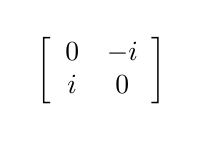
\begin{tikzpicture}
\node[] at (0,0)
     {
       $\left[
         \begin{array}{cc} 0&-i\\i&0\end{array}
             \right]$
       };
\end{tikzpicture}

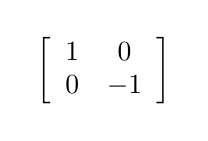
\begin{tikzpicture}
\node[] at (0,0)
     {
       $\left[
         \begin{array}{cc} 1&0\\0&-1\end{array}
             \right]$
       };
\end{tikzpicture}

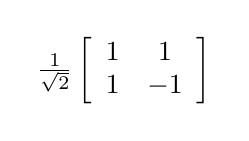
\begin{tikzpicture}
\node[] at (0,0)
     {
       $\frac1{\sqrt2}\left[
         \begin{array}{cc} 1&1\\1&-1\end{array}
             \right]$
       };
\end{tikzpicture}

\end{document}


